\documentclass{article}
\usepackage{graphicx} % Required for inserting images
\usepackage{tikz}
\usetikzlibrary{positioning}
\usepackage{xcolor}   % in your preamble
\definecolor{maroon}{RGB}{128,0,0}
\definecolor{navy}{RGB}{0,0,128}
\usepackage{amsmath}
\usepackage{hyperref}
\usepackage{physics}

\title{$\nu$ral Networks}
\author{Pratik T}
\date{June 2025}

\begin{document}

\maketitle

\section{Project Aim}

Creating a neural network from scratch to predict what number a given handwritten input is.

\section{Structure}

\begin{enumerate}
    \item The input will be a vector of $28\times28 = 784$ elements. This will represent $784$ pixels in the input image. Each pixel will have a grayscale value. The data is from \href{https://www.kaggle.com/datasets/animatronbot/mnist-digit-recognizer}{MNIST}.
    \item There will be 1 hidden layer of 10 elements that initially takes on random values. 
    \item The output layer will also have 10 elements representing the numbers 0 through 9. This layer is also initialized with random values.
\end{enumerate}

\begin{center}
    
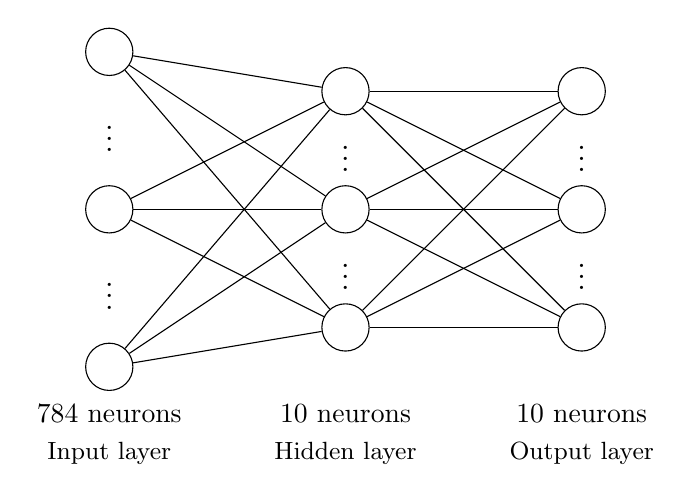
\begin{tikzpicture}[
    neuron/.style={circle, draw, minimum size=6mm},
    ellipsis/.style={font=\large},
    every label/.style={font=\small}]

  % Input layer (900 neurons)
  \node[neuron] (I0) at (0, 2) {};
  \node[neuron] (I1) at (0, 0) {};
  \node[neuron] (I2) at (0,-2) {};
  \node[ellipsis] (Idots) at (0, -1) {\(\vdots\)};
  \node[ellipsis] (Idots) at (0, 1) {\(\vdots\)};
  \node[align=center, label=below:Input layer] at (0,-2.6) {784 neurons};

  % Hidden layer (10 neurons)
  \node[neuron] (H0) at (3, 1.5) {};
  \node[neuron] (H1) at (3, 0) {};
  \node[neuron] (H2) at (3,-1.5) {};
  \node[ellipsis] (Hdots) at (3, -0.75) {\(\vdots\)};
  \node[ellipsis] (Hdots) at (3, 0.75) {\(\vdots\)};
  \node[align=center, label=below:Hidden layer] at (3,-2.6) {10 neurons};

  % Output layer (10 neurons)
  \node[neuron] (O0) at (6, 1.5) {};
  \node[neuron] (O1) at (6, 0) {};
  \node[neuron] (O2) at (6,-1.5) {};
  \node[ellipsis] (Odots) at (6, -0.75) {\(\vdots\)};
  \node[ellipsis] (Odots) at (6, 0.75) {\(\vdots\)};
  \node[align=center, label=below:Output layer] at (6,-2.6) {10 neurons};

  % Connections: Input → Hidden (between real circles)
  \foreach \i in {0,1,2} {
    \foreach \j in {0,1,2} {
      \draw[-] (I\i) -- (H\j);
    }
  }

  % Connections: Hidden → Output (between real circles)
  \foreach \i in {0,1,2} {
    \foreach \j in {0,1,2} {
      \draw[-] (H\i) -- (O\j);
    }
  }

\end{tikzpicture}

\end{center}

\section{Forward Propagation : Perceptron}

\begin{enumerate}
    \item For an input, a perceptron computes its output by applying a linear transform on the input and then passing it through an activation function to introduce nonlinearity. Any multilayer network without an activation will be essentially useless, as it will still be a linear combination. 
    \item \textbf{Linear combination step} 
    \begin{enumerate}
        \item Each neuron in the hidden layer first computes $b+ (x_1\times w_1)+ (x_2\times w_2)+...$. Here $b$ is the bias associated with the neuron, and $w_i$ are the weights associated with the connections between this neuron and a neuron of the preceding layer $x_i$. For a $i\times 1$ column vector $\textbf{x}$, the linear combination output would look like \[ \textbf{W}^T\cdot\textbf{x}+b\] where \textbf{W} is also a vector of dimensions $[i\times 1]$ and $b$ is a number. This is the linear combination output of 1 neuron.
        \item For multiple neurons then the output of the $i^{th}$ neuron for $m$ neurons in the previous $x$ layer is \[z_i = b_{i}+\sum_{j=1}^m w_{ij} x_j\]
    
    \begin{center}
        
    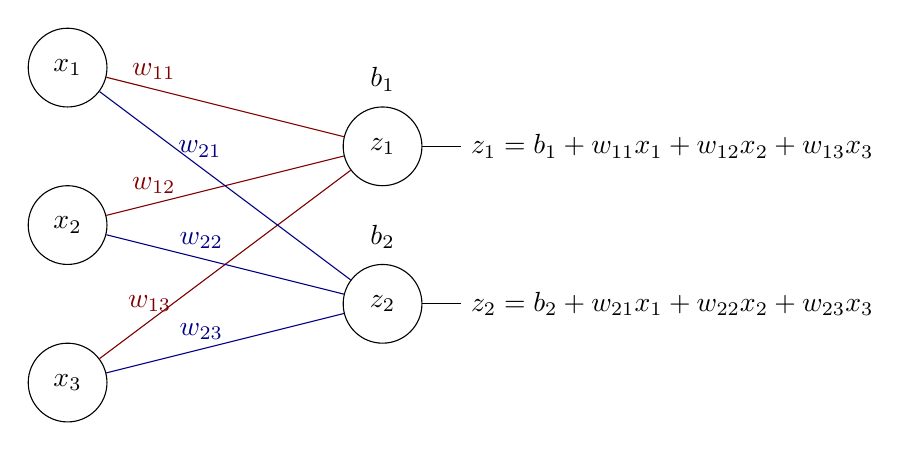
\begin{tikzpicture}[
        neuron/.style={circle, draw, minimum size=10mm},
        ellipsis/.style={font=\large},
        every label/.style={font=\small},
        maroonline/.style={-, draw=maroon},
        navyline/.style={-, draw=navy}
      ]
    
      % Input layer (3 neurons)
      \node[neuron] (I0) at (0, 2) {$x_1$};
      \node[neuron] (I1) at (0, 0) {$x_2$};
      \node[neuron] (I2) at (0,-2) {$x_3$};
    
      % Hidden layer (2 neurons)
      \node[neuron] (H0) at (4, 1) {$z_1$};
      \node[above=2pt of H0] {$b_{1}$};
      \node[neuron] (H1) at (4,-1) {$z_2$};
      \node[above=2pt of H1] {$b_{2}$};
    
      % Connections to H0 (maroon)
      \draw[maroonline] (I0) -- (H0) node[pos=0.2, above, text=maroon] {$w_{11}$};
      \draw[maroonline] (I1) -- (H0) node[pos=0.2, above, text=maroon] {$w_{12}$};
      \draw[maroonline] (I2) -- (H0) node[pos=0.2, above, text=maroon] {$w_{13}$};
    
      % Connections to H1 (navy)
      \draw[navyline] (I0) -- (H1) node[pos=0.4, above, text=navy] {$w_{21}$};
      \draw[navyline] (I1) -- (H1) node[pos=0.4, above, text=navy] {$w_{22}$};
      \draw[navyline] (I2) -- (H1) node[pos=0.4, above, text=navy] {$w_{23}$};
    
      % Outputs
      \draw[-] (H0) -- ++(1,0) node[right] {$z_1 = b_{1} + w_{11}x_1+ w_{12}x_2+ w_{13}x_3$};
      \draw[-] (H1) -- ++(1,0) node[right] {$z_2 = b_{2} + w_{21}x_1+ w_{22}x_2+ w_{23}x_3$};
    
    \end{tikzpicture}
    
    \end{center}

    \begin{equation*}
        \begin{bmatrix}
            z_1\\z_2
        \end{bmatrix} = 
        \begin{bmatrix}
            b_{1}\\b_{2}
        \end{bmatrix} +
                \begin{bmatrix}
            w_{11} & w_{12}\\
            w_{21} & w_{22}\\
            w_{31} & w_{32}
        \end{bmatrix}^T
        \begin{bmatrix}
            x_1 \\ x_2 \\ x_3
        \end{bmatrix}
    \end{equation*}
    \[\vec{z} = \vec{b}+\overset{\leftrightarrow}{W^T}\vec{x}\]
    
    \item $W$ and $b$ are called the weights and biases of the network. Since all neurons are connected, it's called a dense network. The result of the neuron is thus a linear combination of all preceding neurons. 
    \item There are weights and bias matrices associated which each layer. Since our network structure has 2 layers (hidden and output), there's going to be 2 weight matrices and 2 bias vectors.

    \end{enumerate}
    
    \item \textbf{Hidden layer activation}: The linear output of the neuron is then passed through a non-linear function. For now, use ReLU
    \[\mathrm{ReLU}(x_i) = \mathrm{max}(0,x_i)\]
    This is useful when we don't have/want any negative numbers in the output. If an initial neuron does become negative, then the neuron output becomes 0 and this might propagate and give unsatisfactory results. This is called ReLU dying. Another activation is Sigmoid which also gives a value between 0 and 1. But this will be more useful if we only have 1 output.
    \item \textbf{Output Activation}: We want the output of the final layer to be 10 values probabilities which add up to 1. Softmax can be used for this. 
    \[\mathrm{SM(x_i)} = \frac{e^{x_i}}{\sum_j e^{x_j}}\]
    This normalizes the output values so that they add up to 1. 
    
\end{enumerate}

\section{Loss}

\begin{enumerate}
    \item To be able to quantify the performance of a DNN, we need a measure of loss. For this problem, since the output is a vector of probability values, with the desired output being 1 for whatever the input number is and 0 for everything else. Our loss can then be a deviation of the predicted probabilities from the actual probability. Again, the actual probability vector will obviously be all 0s except for the input number which will have a probability of 1. To find the deviations between two probability distributions for binary checks, we can use a cross-entropy loss
    \[\mathcal{L} = -\sum_iy_i\ln(z_i)\]
    where $y_i$ is the actual and $z_i$ is the predicted value.
    Cross-entropy is good for probability distributions as values too far away from the desired value are penalized more harshly.
    \item For outputs which can take on continuous values, losses like mean absolute or mean squared errors make more sense.

\end{enumerate}

\section{Gradient Descent}

\begin{enumerate}
    \item We want to find the optimal values of the weights to minimize the loss function. Since the loss is a function of all the weights of our network, we need to find the local slope in our hyper-dimensional loss landscape. By going in the direction of negative slope, we can then `descent' to a local minimum.
    \item The algorithm is thus as follows: 
        \begin{enumerate}
            \item Initialize weights randomly at step 0
            \item Do a forward pass and compute the loss $\mathcal{L}$ 
            \item Compute the gradient ${\partial \mathcal{L}}/{\partial w}$ where $w$ is a weight (either from the weight matrix, or from the bias)
            \item Update the weights $w = w-\alpha\cdot\frac{\partial \mathcal{L}}{\partial w}$ where $\alpha$ is the step-size (learning rate). The negative comes because we want to go in the opposite direction of the gradient to descent
            \item Repeat till convergence or for set number of iterations
            \item Return the weights after completion to get the `trained' model
        \end{enumerate}

    \item Computing the gradient in a neural network is called back propagation. This is because we start at the output layer and use the chain rule to compute partial derivatives at each network layer to get the net gradient of a loss with a weight parameter. 

\end{enumerate}

\section{Back Propagation}

    \begin{enumerate}
    \item The gradient which will be used to update weights  $w_{i,j}^{(n)}$ is $\partial\mathcal{L}/\partial w_{i,j}^{(n)}$. Let's evaluate this step by step.
    \item Let $g(z)$ be the activation function. Then at a layer $n$ (using Einstein summation convention)

    \[
      x_i^{(n)} = g_i(z^{(n)}) 
      = g_i\!\Bigl(b_i^{(n)} + \sum_k w_{ik}^{(n)}x_k^{(n-1)}\Bigr).
    \]
    Here \(g\) can be \textbf{any} vector activation, so
    \[
      J_{ij}(z^{(n)}) \;\equiv\;\frac{\partial x_i^{(n)}}{\partial z_j^{(n)}}
      \quad\text{(the full Jacobian, not diagonal).}
    \]
    
    \begin{enumerate}
        
        \item \textbf{The weight derivative}:
        \begin{align*}
        \frac{\partial x_i^{(n)}}{\partial w_{pq}^{(n)}}
        &= \sum_{l}
          \frac{\partial x_i^{(n)}}{\partial z_l^{(n)}}
          \,\frac{\partial z_l^{(n)}}{\partial w_{pq}^{(n)}} = 
          \sum_{l}
          J_{il}
          \,\frac{\partial }{\partial w_{pq}^{(n)}}\left[b_l^{(n)} + \sum_k w_{lk}^{(n)}x_k^{(n-1)}\right]\\
        &= J_{i p}(z^{(n)})\,x_q^{(n-1)}.
      \end{align*}
       This is a full 3D tensor.
      
        \item \textbf{The bias derivative}:
        \[
        \frac{\partial x_i^{(n)}}{\partial b_p^{(n)}}
        = \sum_{l} J_{il}\,\frac{\partial z_l}{\partial b_p}
        = J_{i p}(z^{(n)}).
      \]
        
    \end{enumerate}

    \item Now we evaluate the loss gradient. Again, for a layer $n$,

    \begin{enumerate}
        \item \textbf{The weight gradient}:
        \begin{align*}
            \pdv{\mathcal{L}\left(x_i^{(N)}\right)}{w^{(n)}_{pq}} &= \pdv{\mathcal{L}}{x_i^{(N)}}\cdot \pdv{x_i^{(N)}}{w_{pq}^{(n)}}\\
            &= \pdv{\mathcal{L}}{x_i^{(N)}}\cdot \pdv{x_i^{(N)}}{x_j^{(N-1)}}\cdot \pdv{x_j^{(N-1)}}{x_k^{(N-2)}}\cdot \pdv{x_k^{(N-2)}}{x_l^{(N-3)}}...\pdv{x_l^{(n)}}{w_{pq}^{(n)}}
        \end{align*}

        \begin{enumerate}
        \item For the matrix form, let's proceed step by step again. Start at the last layer weights, $n=N$.

        \begin{align*}
        \frac{\partial \mathcal{L}}{\partial w_{pq}^{(N)}}
        &= \sum_i \frac{\partial \mathcal{L}}{\partial x_i^{(N)}}\;\frac{\partial x_i^{(N)}}{\partial w_{pq}^{(N)}}\\
        &= \sum_i \frac{\partial \mathcal{L}}{\partial x_i^{(N)}}\;J_{\,i p}\bigl(z^{(N)}\bigr)\;x_q^{(N-1)}\\
        &= \left[\sum_i \frac{\partial \mathcal{L}}{\partial x_i^{(N)}}\;\frac{\partial x_i^{(N)}}{\partial z_p^{(N)}}\right]\;x_q^{(N-1)}\\
        &= \epsilon_p^{(N)}\;x_q^{(N-1)},
        \end{align*}
        
        The first term is known as the error-signal vector, $\vec{\epsilon}$ and is of dimensionality $p\times 1$, such that the final product again has dimensionality $p\times q$

        \[\pdv{\mathcal{L}}{\overset{\leftrightarrow}{W}^{(N)}} = \vec{\epsilon}^{\ (N)}\cdot \vec{x}^{(N-1)^T}\]

        \item Let's now find the weight gradient for the $N-1$ layer. Remember $x_i^{(N)} = g_i\left(z_i^{(N)}\right)$ and $z_i^{(N)} = b_{1}^{(N)}+\sum_k w_{ik}^{(N)}x_k^{(N-1)}$

        \begin{align*}
            \pdv{\mathcal{L}}{w^{(N-1)}_{pq}} &= \sum_i\sum_j\pdv{\mathcal{L}}{x_i^{(N)}}\cdot \pdv{x_i^{(N)}}{x_j^{(N-1)}}\cdot\pdv{x_j^{(N-1)}}{w_{pq}^{(N-1)}}\\
            &= \sum_i\sum_j\sum_k\pdv{\mathcal{L}}{x_i^{(N)}}\cdot \pdv{x_i^{(N)}}{z_k^{(N)}}\cdot\pdv{z_k^{(N)}}{x_j^{(N-1)}}\cdot J_{j p}\bigl(z^{(N-1)}\bigr)\;x_q^{(N-2)}\\
            &= \sum_{i,j,k}\pdv{\mathcal{L}}{x_i^{(N)}}\cdot J_{ik}^{(N)}\cdot w_{kj}^{(N)}\cdot J_{j p}^{(N-1)}\;x_q^{(N-2)}\\
            &= \left[\sum_{j,k}\epsilon_k^{(N)}\cdot w_{kj}^{(N)}\cdot J_{j p}^{(N-1)}\right]\;x_q^{(N-2)}\\
            &=\epsilon_p^{(N-1)}\;x_q^{(N-2)},
        \end{align*}
        We can write this in matrix notation to again give an output with dimensions of $\overset{\leftrightarrow}{W}^{(N-1)}$
         \[\pdv{\mathcal{L}}{\overset{\leftrightarrow}{W}^{(N-1)}} = \vec{\epsilon}^{\ (N-1)}\cdot\vec{x}^{(N-2)^T}\]


         \item Similarly we can compute this for all the layers, propagating backwards. 

        \item So where is the recursion? It's actually in the error vector of the hidden layers. We can write this as
        \begin{align*}
            \epsilon_p^{(N-1)}&=\sum_{j,k}\epsilon_k^{(N)}\cdot w_{kj}^{(N)}\cdot J_{j p}^{(N-1)}\\
            \epsilon_p^{(n)}&=\sum_{j,k}\epsilon_k^{(n+1)}\cdot w_{kj}^{(n+1)}\cdot J_{j p}^{(n)}\\
            \vec{\epsilon}^{\ (n)} &= \overset{\leftrightarrow}{J}\left(\vec{z}^{\ (n)}\right)^T\left[\overset{\leftrightarrow}{W}^{(n+1)^T}\vec{\epsilon}^{\ (n+1)}\right]
        \end{align*}
        Where in the last step we took a transpose to convert it into a column vector. The output has dimensions $p\times 1$
        \end{enumerate}
        
        \item \textbf{The bias gradient}:

        \begin{align*}
            \pdv{\mathcal{L}}{b^{(N)}_{p}} &= \sum_i\pdv{\mathcal{L}}{x_i^{(N)}}\cdot \pdv{x_i^{(N)}}{b_{p}^{(N)}}\\
            &=\sum_i\pdv{\mathcal{L}}{x_p^{(N)}}\cdot J_{ip}^{(N)}\\
            &=\vec{\epsilon}^{\ (N)}
        \end{align*}
         So the bias gradient is just the error vector. 
    \end{enumerate}

\item Putting it together:

    \begin{center}
    \renewcommand{\arraystretch}{3}
    \begin{tabular}{|c|c|}
    \hline
    \textbf{Weights Gradient} & $ \frac{\partial \mathcal{L}}{\partial w_{pq}^{(n)}} = \epsilon_p^{(n)}\;x_q^{(n-1)}$ \\
    \hline
    \textbf{Bias Gradient} & ${\partial\mathcal{L}}/{\partial{b}_p^{(n)}} = {\epsilon}_p^{\ (n)}$ \\
    \hline
    \textbf{Hidden Layer Error Vector} & $\epsilon_p^{(n)}=\sum_{j,k}\epsilon_k^{(n+1)}\cdot w_{kj}^{(n+1)}\cdot J_{j p}^{(n)}$ \\
    \hline
    \textbf{Boundary Error of Output} & ${\epsilon}_p^{\ (N)} = \sum_i\frac{\partial \mathcal{L}}{\partial x_i^{(N)}}\;J_{\,i p}^{(N)}$ \\
    \hline
    \end{tabular}
    \end{center}
    
\end{enumerate}

\section{A Specific Example}


    Let's compute the gradients for this example of a $N=2$ layer neural network

    \begin{center}
    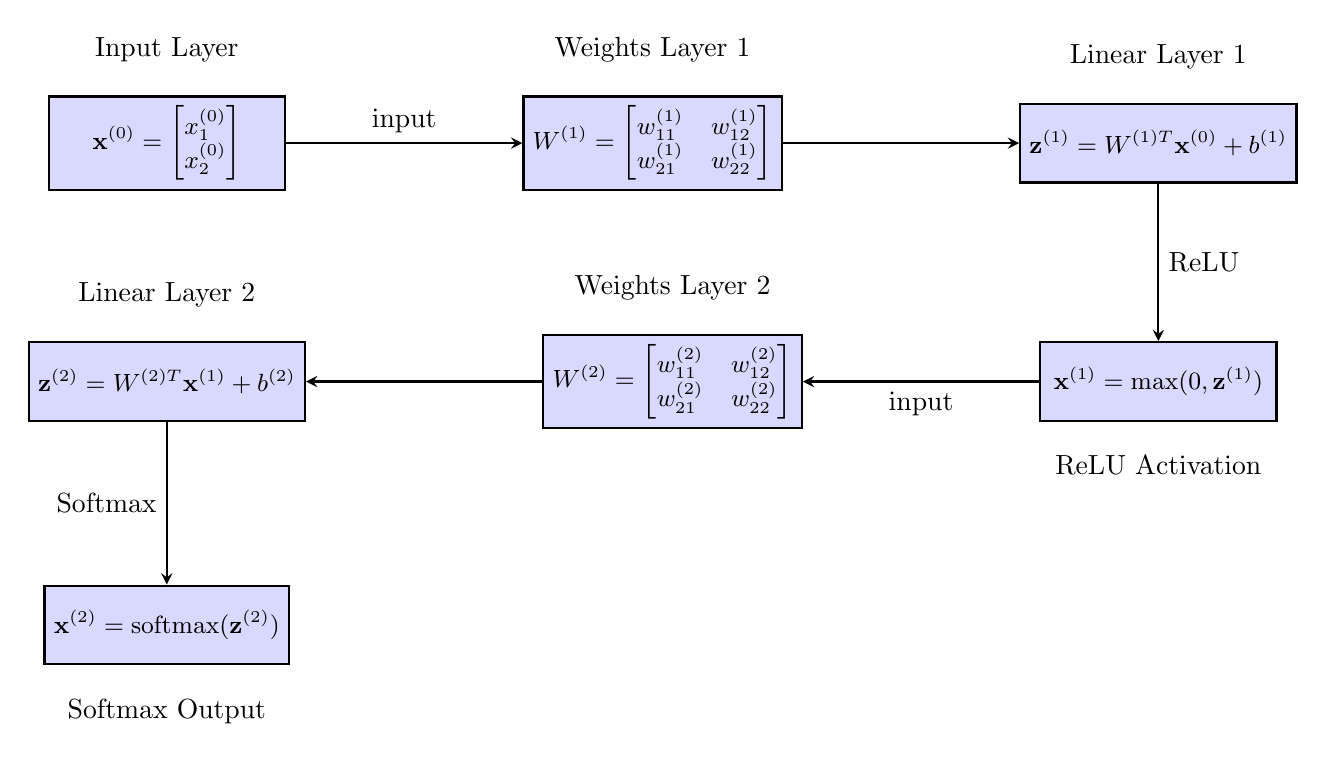
\begin{tikzpicture}[>=stealth, thick,
  vec/.style={draw, minimum width=3cm, minimum height=1cm, fill=blue!15, font=\small, align=center},
  act/.style={font=\footnotesize, sloped, above}
]

% Row 1
\node[vec] (x0) at (0,0) {$\mathbf{x}^{(0)} = \begin{bmatrix} x_1^{(0)} \\ x_2^{(0)} \end{bmatrix}$};
\node[vec, right=3cm of x0] (W1) {$W^{(1)} = \begin{bmatrix} w_{11}^{(1)} & w_{12}^{(1)} \\ w_{21}^{(1)} & w_{22}^{(1)} \end{bmatrix}$};
\node[vec, right=3cm of W1] (z1) {$\mathbf{z}^{(1)} = W^{(1)T} \mathbf{x}^{(0)} + b^{(1)}$};

% Row 2
\node[vec, below=2cm of z1] (x1) {$\mathbf{x}^{(1)} = \max(0, \mathbf{z}^{(1)})$};
\node[vec, left=3cm of x1] (W2) {$W^{(2)} = \begin{bmatrix} w_{11}^{(2)} & w_{12}^{(2)} \\ w_{21}^{(2)} & w_{22}^{(2)} \end{bmatrix}$};
\node[vec, left=3cm of W2] (z2) {$\mathbf{z}^{(2)} = W^{(2)T} \mathbf{x}^{(1)} + b^{(2)}$};

% Row 1 continuation
\node[vec, below=5cm of x0] (x2) {$\mathbf{x}^{(2)} = \mathrm{softmax}(\mathbf{z}^{(2)})$};

% Labels
\node[above=0.3cm of x0] {Input Layer};
\node[above=0.3cm of W1] {Weights Layer 1};
\node[above=0.3cm of z1] {Linear Layer 1};

\node[below=0.3cm of x1] {ReLU Activation};
\node[above=0.3cm of W2] {Weights Layer 2};
\node[above=0.3cm of z2] {Linear Layer 2};

\node[below=0.3cm of x2] {Softmax Output};

% Arrows Row 1 left to right
\draw[->] (x0) -- (W1) node[midway, above] {input};
\draw[->] (W1) -- (z1) node[midway, above] {};
\draw[->] (z1) -- (x1) node[midway, right] {ReLU};

% Arrows Row 2 right to left
\draw[->] (x1) -- (W2) node[midway, below] {input};
\draw[->] (W2) -- (z2) node[midway, below] {};
\draw[->] (z2) -- (x2) node[midway, left] {Softmax};

\end{tikzpicture}
    \end{center}
    
    \begin{center}
    \renewcommand{\arraystretch}{2.5}
    \begin{tabular}{|c|c|}
    \hline
    \textbf{Loss} & $\mathcal{L} = -\sum_i y_i \ln(x_i^{(2)})$ \\
    \hline
    \textbf{Softmax} & $x_i^{(2)} = \dfrac{e^{z_i^{(2)}}}{\sum_j e^{z_j^{(2)}}}$ \\
    \hline
    \textbf{ReLU} & $x_i^{(1)} = \max(0, z_i^{(1)})$ \\
    \hline
    \textbf{Linear} & $z_i^{(n)} = b_{i}^{(n)} + \sum_{j}  w_{ij}^{(n)}x_j^{(n-1)}$ \\
    \hline
    \end{tabular}
    \end{center}

We essentially need to compute the jacobians and loss derivatives. Refer back to the previous table and use $N=2$.  

\begin{enumerate}
    \item Jacobian of Softmax (drop the $z$ superscript): 
    \begin{align*}
    J_{ip}^{(2)} &= \frac{\mathrm{d}x_i^{(2)}}{\mathrm dz_p} = \frac{\mathrm{d}}{\mathrm dz_p}\left[\dfrac{e^{z_i}}{\sum_j e^{z_j}}\right]\\
    &= \dfrac{e^{z_i}\delta_{ip}}{\sum_j e^{z_j}} - \dfrac{e^{z_i}e^{z_p}\delta_{pj}}{\left(\sum_j e^{z_j}\right)^2}\\
    &= x_i^{(2)}\delta_{ip} - x_i^{(2)}x_p^{(2)}\\
    &= x_i^{(2)}\left(\delta_{ip}- x_p^{(2)}\right)
    \end{align*}
    
    \item Derivative of Loss: 
    \begin{align*}
        \mathcal{L}' &= \frac{\mathrm{d}}{\mathrm dx_i^{(2)}}\left[-\sum_j y_j \ln(x_j^{(2)})\right]= -\frac{y_i}{x_i^{(2)}} 
    \end{align*}
    \item Boundary error term: 
    \begin{align*}
        \epsilon_p^{(2)} &= \sum_i -\frac{y_i}{x_i^{(2)}}\cdot x_i^{(2)}\left(\delta_{ip}- x_p^{(2)}\right)\\
        &= -y_p +x_p^{(2)}\sum_i y_i\\
        &= x_p^{(2)} - y_p
    \end{align*}
    Where since $y_i$ are normalised probability values, they add up to 1

    \item Gradients for layer 2:
    \begin{enumerate}
        \item Weights ${\Rightarrow\nabla w_{pq}^{(2)}} = \epsilon_p^{(2)}\;x_q^{(1)}$
    \item Biases $\Rightarrow{\nabla{b}_p^{(2)}} = \epsilon_p^{(2)}$
    \end{enumerate}
    
    \item Jacobian for ReLU:
    \begin{align*}
    J_{jp}^{(1)} &= \frac{\mathrm{d}x_j^{(1)}}{\mathrm dz_p} = \frac{\mathrm{d}}{\mathrm dz_p}\left[\text{max}(0, z_j)\right]\\
    & = \delta_{jp} \iff z_j>0
    \end{align*}

    \item Hidden layer error: 
    \begin{align*}
        \epsilon_p^{(1)}&=\sum_{j,k}\epsilon_k^{(2)}\cdot w_{kj}^{(2)}\cdot J_{j p}^{(1)}\\
        &= \sum_{k}\epsilon_k^{(2)}\cdot w_{kp}^{(2)}\times \left\{\begin{array}{c}
1 ;\ \  z_p^{(1)}>0\\ 0;\ \ z_p^{(1)}\leq0  \end{array} \right.
    \end{align*}
    Here $z_p^{(1)}$ Is the linear output of the layer before activation.

    \item Gradients for layer 1: 
    \begin{enumerate}
        \item Weights ${\Rightarrow\nabla w_{pq}^{(1)}} = \epsilon_p^{(1)}\;x_q^{(0)}$
    \item Biases $\Rightarrow{\nabla{b}_p^{(1)}} = \epsilon_p^{(1)}$
    \end{enumerate}
    
\end{enumerate}

Usually it's much more efficient to pass a batch of inputs at once during training. If the batch is of size $m$, the gradient is an average over all the gradients. So 
    \[\nabla w^{(2)}_{} = \frac{1}{m}\sum_{i=1}^m\epsilon^{(2)}_{p,i} x^{(1)}_{q,i}\]
    The sum can be done directly with a matrix product $x^{(1)}\epsilon^{(2)^T}$. It can be seen as follows (dropping the superscripts): 

    \begin{align*}&
        \begin{bmatrix}
            \epsilon_{11} & \epsilon_{12}&...&\epsilon_{1m}\\
            \epsilon_{21} & \epsilon_{22}&...&\epsilon_{2m}\\
            \vdots & \vdots&...&\vdots\\
            \epsilon_{10,1} & \epsilon_{10,2}&...&\epsilon_{10,m}\\
        \end{bmatrix}\times 
        \begin{bmatrix}
            x_{11} & x_{21}&...&x_{10,1}\\
            x_{12} & x_{22}&...&x_{10,2}\\
            \vdots & \vdots&...&\vdots\\
            x_{1,m} & x_{2,m}&...&x_{10,m}\\ 
        \end{bmatrix} \\&= 
        \begin{bmatrix}
            \epsilon_{11}x_{11}+\epsilon_{12}x_{12}+\cdots+\epsilon_{1m}x_{1,m} & ...&\epsilon_{11}x_{10,1}+\epsilon_{12}x_{10,2}+\cdots+\epsilon_{1m}x_{10,m}\\
            \epsilon_{21}x_{11}+\epsilon_{22}x_{12}+\cdots+\epsilon_{2m}x_{1,m} & ...& \epsilon_{21}x_{10,1}+\epsilon_{22}x_{10,2}+\cdots+\epsilon_{2m}x_{10,m}\\
             \vdots&...&\vdots\\
            \epsilon_{10,1}x_{11}+\epsilon_{10,2}x_{12}+\cdots+\epsilon_{10,m}x_{1,m} &...&\epsilon_{10,1}x_{10,1}+\epsilon_{10,2}x_{10,2}+\cdots+\epsilon_{10,m}x_{10,m}\\ 
        \end{bmatrix}\\
        &= \sum_{i=1}^m\begin{bmatrix}
            \epsilon_{1,i}x_{1,i} & ...&\epsilon_{1,i}x_{m,i}\\
            \epsilon_{2,i}x_{1,i} & ...& \epsilon_{2,i}x_{m,i}\\
             \vdots&...&\vdots\\
            \epsilon_{10,i}x_{1,i} &...&\epsilon_{10,i}x_{m,i}\\ 
        \end{bmatrix} = \sum_{i=1}^m\epsilon^{(2)}_{p,i} x^{(1)}_{q,i}
    \end{align*}
This was also obvious as \[\sum_{i=1}^m x^{(1)}_{q,i}\epsilon^{(2)}_{i,p}\] is the definition of a matrix product.
And we're finally done. Computing these quantities is much simpler as matrices, so that's what we'll write them as. We could also use an input batch which is a matrix where column vectors are joined. This is shown in the next section. 

\section{Algorithm}

\begin{enumerate}
    \item All input will be stored column wise into a matrix. The $x$ input is a $784\times1$ array of pixel data and the $y$ input is a one hot encoded $10\times 1$ array which is 1 for the label corresponding to the input $x$. From this, a single input batch $x^{(0)}$ will be of size $784\times m $ where $m$ is the batch size
    \item Initialize the weight matrices $w^{(1)}$ and $w^{(2)}$ with random values between $-0.5$ and $0.5$. The size of the $w^{(1)}$ is $784\times l$ and $w^{(2)}$ is $l\times l$ where $l$ is the layer size, in our case 10
    \item Initialize the bias matrices $b^{(1)}$ and $b^{(2)}$ of size $l\times 1$ and $l\times 1$.
    \item Perform the first pass to layer 1, which will be a linear transform $z^{(1)} = w^{(1)^T}\cdot x^{(0)} +b^{(1)}$
    \item Pass this through ReLU to get $x^{(1)}$
    \item Apply the linear transform again to get $z^{(2)} = w^{(2)^T}\times x^{(1)}+b^{(2)}$
    \item Pass this through Softmax to get $x^{(2)}$. Normalize the input to softmax so the exponent doesn't blow up.
    \item Now we compare $x^{(2)}$ to our actual value of a one hot encoded column wise $784 \times m$ $y^{(0)}$ matrix of y values. This is done via the boundary error term which we found for the case of the output layer being Softmax and Loss being cross entropy as $\epsilon^{(2)}_{\ \ 784\times m} = x^{(2)}-y^{(0)}$
    \item Using this find the weight gradient for layer 2: $\nabla w^{(2)} = \frac{1}{m}x^{(1)}\epsilon^{(2)^T}$
    \item And the bias gradient for layer 2: $\nabla b^{(2)} = \sum_{i=1}^m\frac{1}{m}\epsilon^{(2)}_i$ 
    \item Find the hidden layer error $\epsilon^{(1)} = w^{(2)^T}\epsilon^{(2)}\odot (1 \iff{z^{(1)}>0}, 0 \ \text{otherwise})$. Here $\odot$ is the Hadamard or element-wise product
    \item Find the weight gradient for layer 1: $\nabla w^{(1)} = \frac{1}{m}x^{(0)}\epsilon^{(1^T)}$
    \item And the bias gradient for layer 1: $\nabla b^{(1)} = \sum_{i=1}^m\frac{1}{m}\epsilon^{(1)}_i$
    \item Update the weights and biases for a set learning rate $\alpha$
    \begin{align*}
        w^{(1)} &= w^{(1)}-\alpha\nabla w^{(1)} & b^{(1)} &= b^{(1)}-\alpha\nabla b^{(1)}\\
        w^{(2)} &= w^{(2)}-\alpha\nabla w^{(2)} & b^{(2)} &= b^{(2)}-\alpha\nabla b^{(2)}
    \end{align*}
    \item Repeat for a set number of epochs. 
    
\end{enumerate}


\end{document}
